\documentclass[11pt]{article} 

\usepackage{amssymb,amsmath}
\usepackage{graphicx}
\usepackage{caption}
\usepackage{subcaption}
\graphicspath{ {./} }

\newcommand{\numpy}{{\tt numpy}}            % tt font for numpy
\newcommand{\scipy}{{\tt scipy}}            % tt font for scipy
\newcommand{\matplotlib}{{\tt matplotlib}}  % tt font for matplotlib

% \topmargin -1in
% \textheight 9in
% \oddsidemargin  -.25in
% \evensidemargin -.20in
% \textwidth 7in

% \topmargin -1in
% \textheight 8.5in
% \oddsidemargin  -0.25in
% \evensidemargin -0.20in
% \textwidth 7in

\topmargin 0in
\textheight 7.5in
\oddsidemargin  -.05in
\evensidemargin 0in
\textwidth 6.5in

\begin{document}

$$\mbox{\Large \bf CS 111: Homework 9: Due by 11:59 pm Tuesday, December 7, 2021}$$
\par\smallskip\noindent
{\bf Submit your paper as one PDF file,
and tell GradeScope which page(s) each problem is on.
If you worked with a partner, 
you must each separately write up and turn in your own homework paper, 
and report the name of your partner.
No groups of more than two.
}

\par\bigskip\noindent
{\bf 1.}
Newton's method is often used with $n=1$ to compute 
values of nonlinear functions like $\sqrt a$. 
To solve $x^2-a=0$, we integrate $x^2-a$ and see that if we define
$$f(x) = x^3/3-ax,$$ 
then at $x=\mbox{argmin} f(x)$ (subject to $x\ge 0$, where $f$ is convex), 
we have $x^2-a = f^\prime(x) = \nabla f(x) = 0$,
so minimizing $f(x)$ computes $x=\sqrt a$.
In the case $n=1$ the Hessian matrix $H$ is just $f^{\prime\prime}(x) = 2x$,
and the Newton iteration is
\begin{align}
x_{k+1} &= x_k - f^\prime(x_k)/f^{\prime\prime}(x_k) \\
        &= x_k - (x_k^2-a)/(2x_k) \\
        &= x_k - x_k/2 +a/(2x_k) \\
        &= \frac{1}{2}\Big(x_k + \frac{a}{x_k}\Big).
\end{align}

\par\medskip\noindent
{\bf 1.1} 
Compute $\sqrt 4$ by Newton's method, starting with $x_0=1$.
Display a table of $k$, $x_k$, and $x_k^2$ for $k=0,1,2,\ldots$\,.
As always, show your python code.
How many iterations does it take to get 4 correct digits?
8 correct digits? 16 correct digits?

\par\medskip\noindent
{\bf 1.2} 
Repeat for $\sqrt 2$, 
displaying the same table and answering the same questions.

\par\bigskip\noindent
{\bf 2.1}
Suppose the East Beach shoreline is the $x$-axis, 
so the beach is all points $(x,y)$ with $y\ge 0$ and 
the ocean is all points with $y<0$.
A lifeguard is positioned at $(x,y) = (0,20)$, that is, 
20 meters north of the beach on the line $x=0$.
The lifeguard sees a swimmer in distress at $(x,y)=(80,-40)$,
that is, 40 meters out to sea and 80 meters east of the lifeguard.

\begin{figure}[t]
\centering
\begin{minipage}{.5\textwidth}
  \centering
  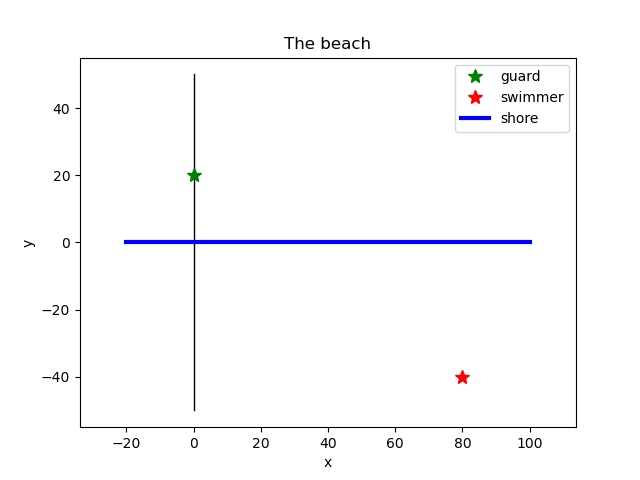
\includegraphics[width=.65\linewidth]{StraightBeach}
  \captionof{figure}{Straight beach (2.1)}
  \label{fig:geometric}
\end{minipage}%
\begin{minipage}{.5\textwidth}
  \centering
  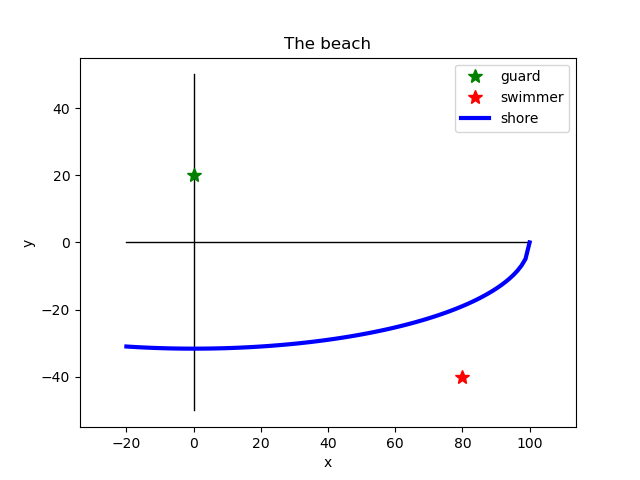
\includegraphics[width=.65\linewidth]{CurvedBeach}
  \captionof{figure}{Curved beach (2.2)}
  \label{fig:spectral}
\end{minipage}
\end{figure}

If the lifeguard runs at a speed of 5 meters/second and swims 
at 1 meter/second, what is the optimal path for the lifeguard
to reach the swimmer in the shortest possible time? 
The lifeguard will run in a straight line to a point $(x,0)$, 
and then swim in a straight line from there to the point $(80,-40)$.
Formulate an optimization problem (in $n=1$ dimension) whose solution is
the point $x$ along the shoreline at which the lifeguard should
enter the water. You may solve the optimization problem either
exactly with pen and paper and calculus, 
or by using one of the solvers from the class demos. 
You might want to try {\tt scipy.optimize.minimize}
with {\tt method='Newton-CG'} or {\tt 'BFGS'}, 
or {\tt cs111.gradient\_descent}
with some hand-tuning of the learning rate.
In any case, report what you find and explain in detail
how you arrived at the optimal value of $x$.

Draw a diagram showing the beach, the lifeguard, the swimmer, 
and the optimal path, with the various distances labelled. 
You can make the drawing either by hand or with matplotlib.
Using the optimal path, 
how many seconds will it take the lifeguard to reach the swimmer?

\par\medskip\noindent
{\bf 2.2}
Same problem as above, but now the shoreline is curved:
Instead of the line $y=0$, the shoreline is the partial ellipse
$y = -\sqrt{1000-x^2/10}$.
Again, formulate a 1-dimensional optimization problem that minimizes the 
time to reach the swimmer over all possible $x$ coordinates at which
the lifeguard could enter the water.
(Now, of course, for any given $x$, the lifeguard will enter the
water at the point $(x,y)$.)
Solve the optimization problem for $x$ using any of the solvers
we demoed in class (feel free to try any of them), 
and report on what you find.

At what point $(x,y)$ does the lifeguard enter the water?
How many seconds does it take the lifeguard to reach the swimmer?
Draw a diagram as before.

\par\bigskip\noindent
{\bf 3.}
Recall the definition of a convex function:
A function $f$ from $\mathbb{R}^n$ to $\mathbb{R}$ is {\em convex} if,
for all $x$ and $y$ in $\mathbb{R}^n$ and all $0\le\alpha\le 1$,
$$\alpha f(x) + (1-\alpha)f(y) \ge f(\alpha x + (1-\alpha)y),$$
that is, every chord is above the function values.

\par\medskip\noindent
{\bf 3.1.}
Assume that functions $f$ and $g$ are both convex.
Prove that the function $h(x)=\max(f(x),g(x))$ is convex
by starting with the definition of convexity for $f$ and $g$ 
and giving a rigorous mathematical argument to show that $h$
satisfies the definition as well.

\par\medskip\noindent
{\bf 3.2.}
Give an example of two convex functions $f$ and $g$ for which
the function $\min(f,g)$ is not convex.
Give values of $x$, $y$, and $\alpha$ for which the definition
is not satisfied, and show the computation that proves it is not.

\end{document}
